%%----------------------------------------------------------------------------
%% Presentatie HoGent Bedrijf en Organisatie
%%----------------------------------------------------------------------------
%% Auteur: Bert Van Vreckem [bert.vanvreckem@hogent.be]
%% Auteur: Wim Goedertier [wim.goedertier@hogent.be]

\documentclass{beamer}

%==============================================================================
% Aanloop
%==============================================================================

%---------- Packages ----------------------------------------------------------

\usepackage{graphicx,multicol}
\usepackage{comment,enumerate,hyperref}
\usepackage{amsmath,amsfonts,amssymb}
\usepackage{tikz}
\usepackage[english]{babel}
\usepackage[utf8]{inputenc}
\usepackage{multirow}
\usepackage{eurosym}
\usepackage{listings}
\usepackage[T1]{fontenc}
\usepackage{lmodern}
\usepackage{textcomp}

%---------- Configuratie ------------------------------------------------------

\usetikzlibrary{arrows,shapes,backgrounds,positioning,shadows}

\usetheme{hogent}

%---------- Commando-definities -----------------------------------------------

\newcommand{\tabitem}{~~\llap{\textbullet}~~}

%---------- Info over de presentatie ------------------------------------------

\title[Intro]{Research techniques -- Intro}
\author{Wim Goedertier (wim.goedertier@hogent.be)  Jens Buyse, Bert {Van Vreckem}, Wim {De Bruyn}}
\date{AY 2017-2018}

%==============================================================================
% Inhoud presentatie
%==============================================================================

\begin{document}

%---------- Front matter ------------------------------------------------------

% Dia met het HoGent logo
\HoGentLogo

% Titeldia met faculteitslogo
\titleframe

%---------- Inhoud ------------------------------------------------------------

% Dia voor sectiekop, voorbeeld met een afbeelding onderaan de pagina
\section{1}

\sectionframelogo{Research techniques}

\begin{frame}{Research techniques}

  \scaledimg{img/intro-01.jpg}
\end{frame}

\begin{frame}{Examples of bad research}

  \scaledimgvert{img/intro-02.png}{img/intro-03.png}
\end{frame}

\begin{frame}{Examples of bad research}

  \scaledimg{img/intro-04.png}
\end{frame}

\begin{frame}{Examples of bad research}

  \scaledimg{img/intro-05.jpg}
\end{frame}

\begin{frame}
  \frametitle{Examples of bad research}

  \scaledimg{img/intro-10.jpg}
\end{frame}

\begin{frame}{Examples of bad research}
	
	\scaledimg{img/intro-nva.jpg}
  
  \tiny \textit{Government spending as percentage of GDP has declined last year, but not as spectacularly as a graph of N-VA (Flemish nationalist and liberal conservative party) suggests. Professor Economics Tom Verbeke noticed it and criticised the party. ``A student that pulls tricks like this would have a hard time justifying himself''}
\end{frame}

\section{2}
\sectionframelogo{Course organisation}

\begin{frame}{Overview course topics}

\begin{table}[h]
\begin{tabular}{l|l}
  \multirow{2}{*}{\textbf{Introduction}} &
     \tabitem Course introduction \\
   & \tabitem Data input \\

  \hline
  \multirow{2}{*}{\textbf{Univariate statistics}} &
      \tabitem Basic summary statistics \\
    & \tabitem Simple graphs\\

  \hline
  \multirow{2}{*}{\textbf{Bivariate statistics}} &
      \tabitem Simple graphs \\
    & \tabitem Correlation and regression\\

  \hline
  \textbf{Sampling and} & \tabitem Population\\
  \textbf{probability distribution}  & \tabitem Sample\\
    & \tabitem The normal distribution\\

  \hline
  \textbf{Hypothesis tests and} & \tabitem Testing hypotheses \\
  \textbf{Chi-square test}     & \tabitem $z$-test, $t$-test\\
                                 & \tabitem $\chi^{2}$-test\\
  \hline
  \textbf{Time series} & \tabitem Mathematicel models \\
                       & \tabitem Moving average \\
                       & \tabitem Exponential smoothing \\
\end{tabular}
\end{table}
\end{frame}

\begin{frame}{Materials used}

  \begin{itemize}
    \item Lecture slides
      \begin{itemize}
        \item contain graphs, tables, \ldots discussed in the lectures
      \end{itemize}
    \item Lectures, notes on black-/whiteboard
      \begin{itemize}
        \item Follow the lectures \textbf{actively}!
        \item \textbf{Take notes!}
      \end{itemize}
    \item Course syllabus
  \end{itemize}

  \brightbox{Follow the lectures and \textcolor{HoGentAccent6}{take notes}}
  
  \begin{center}
    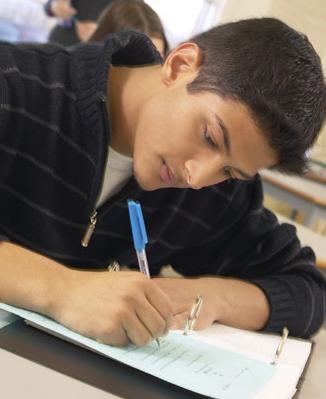
\includegraphics[height=3cm]{img/intro-06.jpg}
  \end{center}

\end{frame}

\begin{frame}{Software}
    
    \begin{itemize}
        \item Git revision control system:
        \begin{itemize}
            \item Git client
            \item Github account
        \end{itemize}
        \item {\LaTeX} typesetting system:
        \begin{itemize}
            \item MikTeX/MacTeX/Texlive
            \item TexStudio (or another editor)
            \item JabRef bibliographic reference manager
        \end{itemize}
        \item Statistics software: R, RStudio Desktop
    \end{itemize}

    \centering
    All required software is free/open source
\end{frame}

\begin{frame}{Course organisation}

  \begin{itemize}
    \item Lectures
      \begin{itemize}
        \item Theoretical foundations
      \end{itemize}
    \item Seminar/practice sessions
      \begin{itemize}
        \item Expanding on knowledge
        \item Exercises
        \item Learning to use the software
      \end{itemize}
    \item Guided independent learning
      \begin{itemize}
        \item Group assignments
        \item ``Passive'' coaching
      \end{itemize}
  \end{itemize}
\end{frame}

\begin{frame}{Course evaluation}

  \begin{itemize}
    \item First exam session (May, June)
      \begin{itemize}
        \item Non-period bound evaluation (during semester): 30\% of total score
          \begin{itemize}
            \item Group assignment, conducting empirical research
          \end{itemize}
        \item Period bound evaluation (exam): 70\% of total score
          \begin{itemize}
            \item Written exam ``closed book'' (theory)
            \item Written exam with use of own laptop (excersises)
          \end{itemize}
      \end{itemize}
    \item Second exam session (August, September)
      \begin{itemize}
        \item Non-period bound: 30\% (score taken from first period)
        \item Period bound: 70\% (new exam, similar to first period)
      \end{itemize}
    \end{itemize}

  \begin{center}
    
\includegraphics[height=3cm]{img/intro-07}
  \end{center}
Study during the entire semester. It's the best way to process the material.
\end{frame}

\begin{frame}
  \frametitle{NPE: Case research process}

  \brightbox{Performance comparison between databases}

  \begin{enumerate}
    \item Reading a scientific paper
    \item Reproduce experiments
    \item Adjust research question, delimit and settle on specific goals
    \item Perform controlled experiments
    \item Collect data (statistically sound), draw conclusions
    \item Write report/paper
  \end{enumerate}

  Assignment is published on Chamilo, under Assignments (Opdrachten)
\end{frame}


%---------- Back matter -------------------------------------------------------

\end{document}
